\documentclass[twocolumn,norwegian]{article}
\usepackage{hyperref}
\hypersetup{colorlinks=true}
\usepackage{titling}
\usepackage{graphicx}
\usepackage{amsmath}
\usepackage[caption=false,font=normalsize,labelfont=sf,textfont=sf]{subfig}
\graphicspath{{figures/}}

%\setlength{\droptitle}{-1cm} 

%opening
\title{TEK9020 - Prosjektoppgave 2}
\author{Kristoffer Langstad \\ kristoffer.langstad@its.uio.no}
\date{}

\begin{document}
	
	\maketitle
	
	\section{Introduksjon}
	I denne oppgaven er målet å se hvordan en klassifikator kan brukes for å gjøre en segmentering av bilder for å skille mellom bestemte fysiske objekter i bildene. Segmentering er ofte brukt som en forhåndsbehandling av bilder for å forenkle innholdet før videre bildeanalyse. I dette tilfellet skal det gjøres ved å klassifisere hver enkelt piksel i RGB-bilder inn i ønskede klasser utifra farge og intensitet i bildene. Klassifikatoren som brukes er minimum feilrate metoden med normalfordelings antagelse. Først testes klassifikatoren ved å bruke et bilde til både trening og testing. Deretter brukes to nye bilder der ett brukes til trening og det andre til testing. Det ses også på hva som skjer dersom pikslene i bildene først blir normalisert, og hva dette har å si for segmenteringen. Resultatene blir til slutt presentert og diskutert. Programmeringen utføres i Python (~\ref{Appendix:Kode}).


	\section{Metode}
	\subsection{Datasett}
	Det brukes totalt tre bilder til trening og testing av minimum feilrate klassifikatoren. Bildene inneholder tre objekter som skal klassifiseres og segmenteres av klassifikatoren både med og uten normaliserte RGB-verdier.
	
	Bilde 1 (Fig.~\ref{subfig:Bilde1}) består av tre objekter; grønn og rød paprika og grønn chili. Dette bildet brukes til både trening og testing av klassifikatoren for å se at klassifikatoren fungerer som den skal for den gitte segmenteringsoppgaven. Bilde 2 og 3 (Fig.~\ref{subfig:Bilde2} og~\ref{subfig:Bilde3}) består av en blå og en rød ringperm og bakgrunn som blir de tre forskjellige klassene som skal segmenteres. I dette tilfellet blir Bilde 2 brukt til kun trening, mens Bilde 3 blir brukt kun til testing. 
	
	\begin{figure*}[ht!]
		\centering
		\subfloat[Bilde 1]{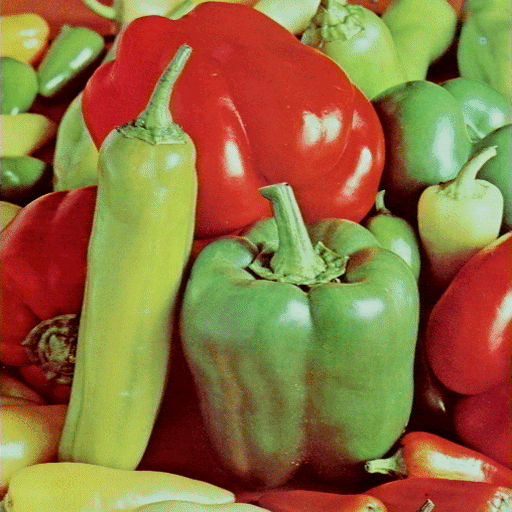
\includegraphics[width=0.3\linewidth,height=0.192\textheight]{../data/Bilde1.png}
		\label{subfig:Bilde1}}
		%\hfil
		\subfloat[Bilde 2]{\includegraphics[width=0.3\linewidth]{../data/Bilde2.png}
		\label{subfig:Bilde2}}
		\subfloat[Bilde 3]{\includegraphics[width=0.3\linewidth]{../data/Bilde3.png}
		\label{subfig:Bilde3}}
		\caption{De tre bildene som brukes til trening og testing av klassifikatoren. \label{fig:Datasett}
		}
	\end{figure*}

	\subsection{Eksperimenter}
	Først velges det ut tre rektangulære områder av passende størrelser som skal brukes som treningssampler for de tre klassene i treningsbildene. Pikslene i diss rektangulære områdene blir brukt som treningssampler for de gitte klassene som skal segmenteres. Når klassifikatoren har trent på disse treningssamplene, skal den segmentere eller tilegne pikslene i testbildet utifra klassene som gitte fargekoder og visualiseres. Dette gjøres for begge treningssituasjonene med bare Bilde 1, og med Bilde 2 og 3 som nevnt tidligere.

	Segmentering kan være mottakelig for feil dersom det er variasjoner i intensitet i bildene, f.eks. lys/skygge, reflekser osv. Derfor blir det også prøvd ut å normalisere RGB-verdiene for å gjøre klassifikatoren mer robust. I dette tilfellet blir normaliserte tristimulusverdier brukt for å normalisere RGB-verdiene i ved transformasjonen:
	\begin{equation*}
		t_1 = \frac{R}{R+G+B}, t_2=\frac{G}{R+G+B}, t_3=\frac{B}{R+G+B}
	\end{equation*}
	I dette tilfellet blir transformasjonene av de tre egenskapene lineært avhengige av hverandre. Dette vil gi en feil i minimum feilrate klassifikatoren siden determinanten til kovariansmatrisene blir null. Derfor blir kun de to første egenskapene $t_1$ og $t_2$ brukt for å unngå denne feilen, i tillegg til at å bruke $t_3$ er unødvendig på grunn av den lineære avhengigheten for egenskapene. De normaliserte bildene blir så brukt til å trenes og testes på som gjort tidligere, med de samme rektangulære treningsområdene.


	\section{Resultater}
	\subsection{Segmentering Bilde 1}
	I det første tilfellet ble det valgt følgende treningsområder markert i blått som vist i Figur~\ref{fig:TreningBilde1} som dekker de tre klassene som er i bildet. Der ser vi treningssamplene for Bilde 1 uten (Fig.~\ref{subfig:Bilde1_Trening}) og med normaliserte RGB-verdier (Fig.~\ref{subfig:Bilde1_Trening_norm}).

	\begin{figure}[ht!]
		\centering
		\subfloat[Original]{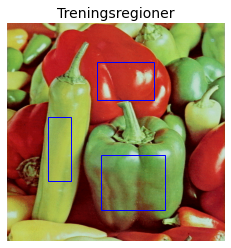
\includegraphics[width=0.5\linewidth]{Trening_paprika.png}
			\label{subfig:Bilde1_Trening}}
		%\hfil
		\subfloat[Normalisert]{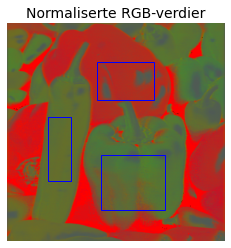
\includegraphics[width=0.5\linewidth]{Trening_paprika_norm.png}
			\label{subfig:Bilde1_Trening_norm}}
		\caption{Markerte treningsområdene for Bilde 1 uten og med normaliserte RGB-verdier. \label{fig:TreningBilde1}}
	\end{figure}

	Med disse treningsområdene ble klassifikatoren trent opp til å klassifisere RGB-verdiene til objektene i Bilde 1 med farger; grønn for grønn chili, gul for grønn paprika og magenta for rød paprika.
	
	\begin{figure}[ht!]
		\centering
		\subfloat[Original]{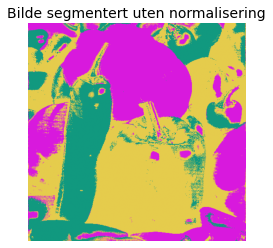
\includegraphics[width=0.5\linewidth]{Test_paprika.png}
			\label{subfig:Bilde1_Test}}
		%\hfil
		\subfloat[Normalisert]{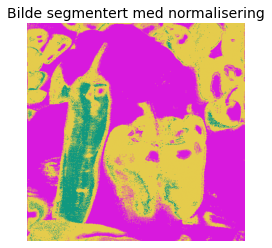
\includegraphics[width=0.5\linewidth]{Test_paprika_norm.png}
			\label{subfig:Bilde1_Test_norm}}
		\caption{Segmenterte bilder av Bilde 1 for originale (venstre) og normaliserte (høyre) RGB-verdier. \label{fig:TestBilde1}}
	\end{figure}

	\subsection{Segmentering Bilde 2 og 3}
	Samme fremgangsmåte ble gjennomført for Bilde 2 og 3 som for Bilde 1, bare med separate trening og test bilder. I Figur~\ref{fig:TreningBilde2} er de markerte treningsområdene for Bilde 2 for rød og blå ringperm og bakgrunn markert med blå rektangler. Her blir treningsområdene basert på hovedfargene til objektene, så farger som metall og ark på permene blir ikke trent på. Figur~\ref{subfig:Bilde2_Trening} og~\ref{subfig:Bilde2_Trening_norm} er de originale og normaliserte RGB-verdiene brukt til trening av ringpermene, respektivt.
	
	\begin{figure}[ht!]
		\centering
		\subfloat[Original]{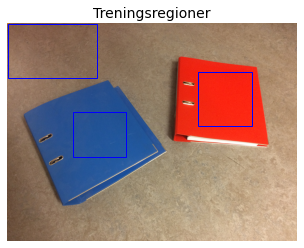
\includegraphics[width=0.5\linewidth]{Trening_permer.png}
			\label{subfig:Bilde2_Trening}}
		%\hfil
		\subfloat[Normalisert]{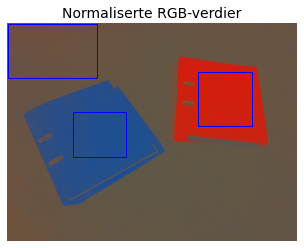
\includegraphics[width=0.5\linewidth]{Trening_permer_norm.png}
			\label{subfig:Bilde2_Trening_norm}}
		\caption{Markerte treningsområdene for Bilde 2 uten og med normaliserte RGB-verdier. \label{fig:TreningBilde2}}
	\end{figure}

	I Figur~\ref{fig:TestBilde3} er resultat av segmenteringene av Bilde 3 med samme klasser som treningen av Bilde 2, men bildet er tatt fra en annen vinkel, for originale (Fig.~\ref{subfig:Bilde3_Test}) og normaliserte (Fig.~\ref{subfig:Bilde3_Test_norm}) RGB-verdier. Bilde 3 er testet uavhengig av treningen av Bilde 2.
	
	\begin{figure}[ht!]
		\centering
		\subfloat[Original]{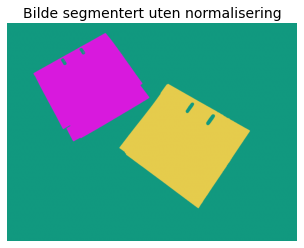
\includegraphics[width=0.5\linewidth]{Test_permer.png}
			\label{subfig:Bilde3_Test}}
		%\hfil
		\subfloat[Normalisert]{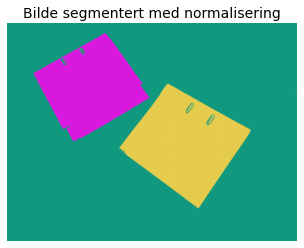
\includegraphics[width=0.5\linewidth]{Test_permer_norm.png}
			\label{subfig:Bilde3_Test_norm}}
		\caption{Segmenterte bilder av Bilde 3 for originale (venstre) og normaliserte (høyre) RGB-verdier. \label{fig:TestBilde3}}
	\end{figure}


	\section{Diskusjon}
	Ved å sammenligne resultatene av de normaliserte RGB-verdiene i Figur~\ref{fig:TreningBilde1} og hvordan dette påvirker segmenteringen av grønnsakene~\ref{fig:TestBilde1}, så er det tydelig at normaliseringen påvirker hvordan klassifikatoren håndterer segmenteringen av grønnsakene. Hovedfargene i treningssamplene for grønnsakene er grønn og rød. Dette gjør at klassifikatoren ikke helt vet hva den skal gjøre med refleksjon og skygge. Med de originale RGB-verdiene så blir skyggene klassifisert som grønn paprika, mens for de normaliserte RGB-verdiene så blir skyggene klassifisert som rød paprika. Så fra normaliseringen ser vi at skyggene får en mer rødaktig farge, mens de tidligere lå nærmere den mørkere grønne fargen. Dette gjør at formen på de grønne grønnsakene blir mer tydeligere segmentert, men på bekostning av de røde paprikaene siden vi kun har tre klasser det kan segmenteres i. Refleksjonene av lys blir i begge tilfeller klassifisert som rød paprika.
	
	Det er ikke stor forskjell mellom grønn paprika og grønn chili, det er litt forskjell i intensitet og nyanse som klassifikatoren har noe trøbbel med å segmentere riktig. Det virker som om etter normaliseringen at det blir noe vanskeligere å klassifisere riktig mellom de to. Selv om det blir lettere å skille mellom grønn og rød, så kan det se ut som om grønnfargene blir nærmere hverandre i RGB-verdier når de har blitt normalisert som fører til litt mer feilklassifisering av chili som paprika.

	Sammenlignet med grønnsakene, så har ikke RGB normaliseringen like mye å si for ringpermene i Figur~\ref{fig:TreningBilde2} og~\ref{fig:TestBilde3}. Her er det både mindre variasjon i intensitet med lite skygger og refleksjon, og det er større avstand i RGB-verdiene mellom de to permene og bakgrunnen som gjør det lettere for klassifikatoren å segmentere riktig. Den største forskjellen er mest tydelig på metallet på den røde ringpermen som blir segmentert litt mer gul etter normaliseringen. Dette er nok på grunn av at vinkelen mellom de to originale bildene har forskjellig refleksjon i metallet som påvirker normaliseringen, og dermed segmenteringen i etterkant. Det er tydelig at normalisering og segmentering er avhengig av variasjonen i intensiteter og RGB-verdiene til objekter i bildene for hvordan klassifiseringen blir med minimum feilrate metoden.


	\section{Konklusjon}
	Resultatene av segmenteringen med og uten normaliserte RGB-verdier har vist å gjøre stor forskjell når det gjelder store variasjoner i intensitet som lys og refleksjon i bildene. For bildene med grønnsakene ble det større forbedring av segmenteringen etter at bildet hadde blitt normalisert, enn for ringpermene med uten store variasjoner. For grønnsakene ble det mer tydelig grenser mellom objektene som ble klassifisert.
	
	I bildene med ringpermene så er det også større spredning i RGB-verdiene for fargene som er mer ulike hverandre enn for grønnsakene. For grønnsakene med forskjellige grønnfarger så var det lettere for klassifikatoren å klassifisere feil siden de var mer like hverandre, enn for blå og rød ringperm som er veldig ulike hverandre i RGB-verdier.
	
	\appendix
	\section{Python kode}
	\label{Appendix:Kode}
	Koden som er brukt i dette prosjektet kan bli funnet i GitHub på: \url{https://github.com/krilangs/TEK9020/tree/main/Project2}
	
\end{document}
